\chapter{Appendix -- Instability of Value Function Learning}

\section{Implementation details and hyperparameters} \label{app:impl}

We employ two commonly used implementations, one for fast iterations on priming experiments (\href{https://github.com/denisyarats/pytorch\_sac}{https://github.com/denisyarats/pytorch\_sac}) and one for scaling up our experiments to high update ratios (\href{https://github.com/proceduralia/high\_replay\_ratio\_continuous\_control}{https://github.com/proceduralia/high\_replay\_ratio\_continuous\_control}). All experiments in the main sections use default hyperparameters of the high update ratio codebase  unless otherwise specified with minor exceptions.

\begin{table}[H]
    \parbox[t]{.45\linewidth}{
    \label{tab:sharedhparam}
    \centering
    \caption{Shared hyperparameters between priming and high-UTD implementations}
    \begin{tabular}{ | m{3.5cm} | m{2cm}| }
      \hline
      Optimizer & Adam \\ 
      \hline
      Adam $\beta_1$ & $0.9$ \\ 
      \hline
      Adam $\beta_2$ & $0.999$ \\ 
      \hline
      Adam $\varepsilon$ & $1e-8$ \\ 
      \hline
      Actor Learning Rate & $4e-3$ \\ 
      \hline
      Critic Learning Rate & $4e-3$ \\ 
      \hline
      Temp. Learning Rate & $3e-4$ \\ 
      \hline
      Batch Size
      & $256$ \\ 
      \hline
      $\gamma$ & $0.99$ \\
      \hline
      $\tau$ & $0.005$ \\
      \hline
      \# critics & $2$ \\
      \hline
      \# critic layers & $2$ \\
      \hline
      \# actor layers & $2$ \\
     \hline
      critic hidden dim & $256$ \\
     \hline
      actor hidden dim & $256$ \\
     \hline
    \end{tabular}
    \label{tab:shared}
    }
    \hfill
    \parbox[t]{.55\linewidth}{
    \centering
    \caption{Differing hyperparameters between priming and high-UTD implementations}
    \begin{tabular}{ |m{2cm} | m{2.5cm} |  m{2.5cm}| }
     \hline
     & Priming & High UTD \\
     \hline\hline
     Initial \newline temperature & $0.1$ & $1.0$ \\
     \hline
     Target \newline entropy & -action\_dim & -action\_dim / 2 \\
     \hline
     actor log \newline std bounds & [-5, 2] & [-10, 2] \\
     \hline
    \end{tabular}
    }
\end{table}


\section{Additional experimental results} \label{app:exp}

\subsection{Returns on all environments} \label{app:exp_ret}

\begin{figure}[H]
\centering
    \begin{subfigure}[b]{0.8\textwidth}
        \centering
        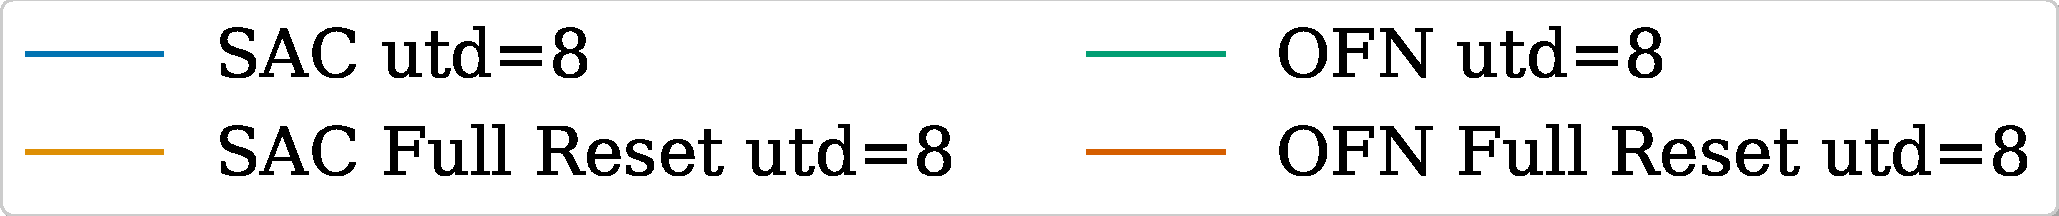
\includegraphics[height=0.8cm]{figures/dissecting/main_exp/utd_8_return_legend.pdf}
    \end{subfigure}\\%
    \begin{subfigure}[b]{1\textwidth}
        \centering
        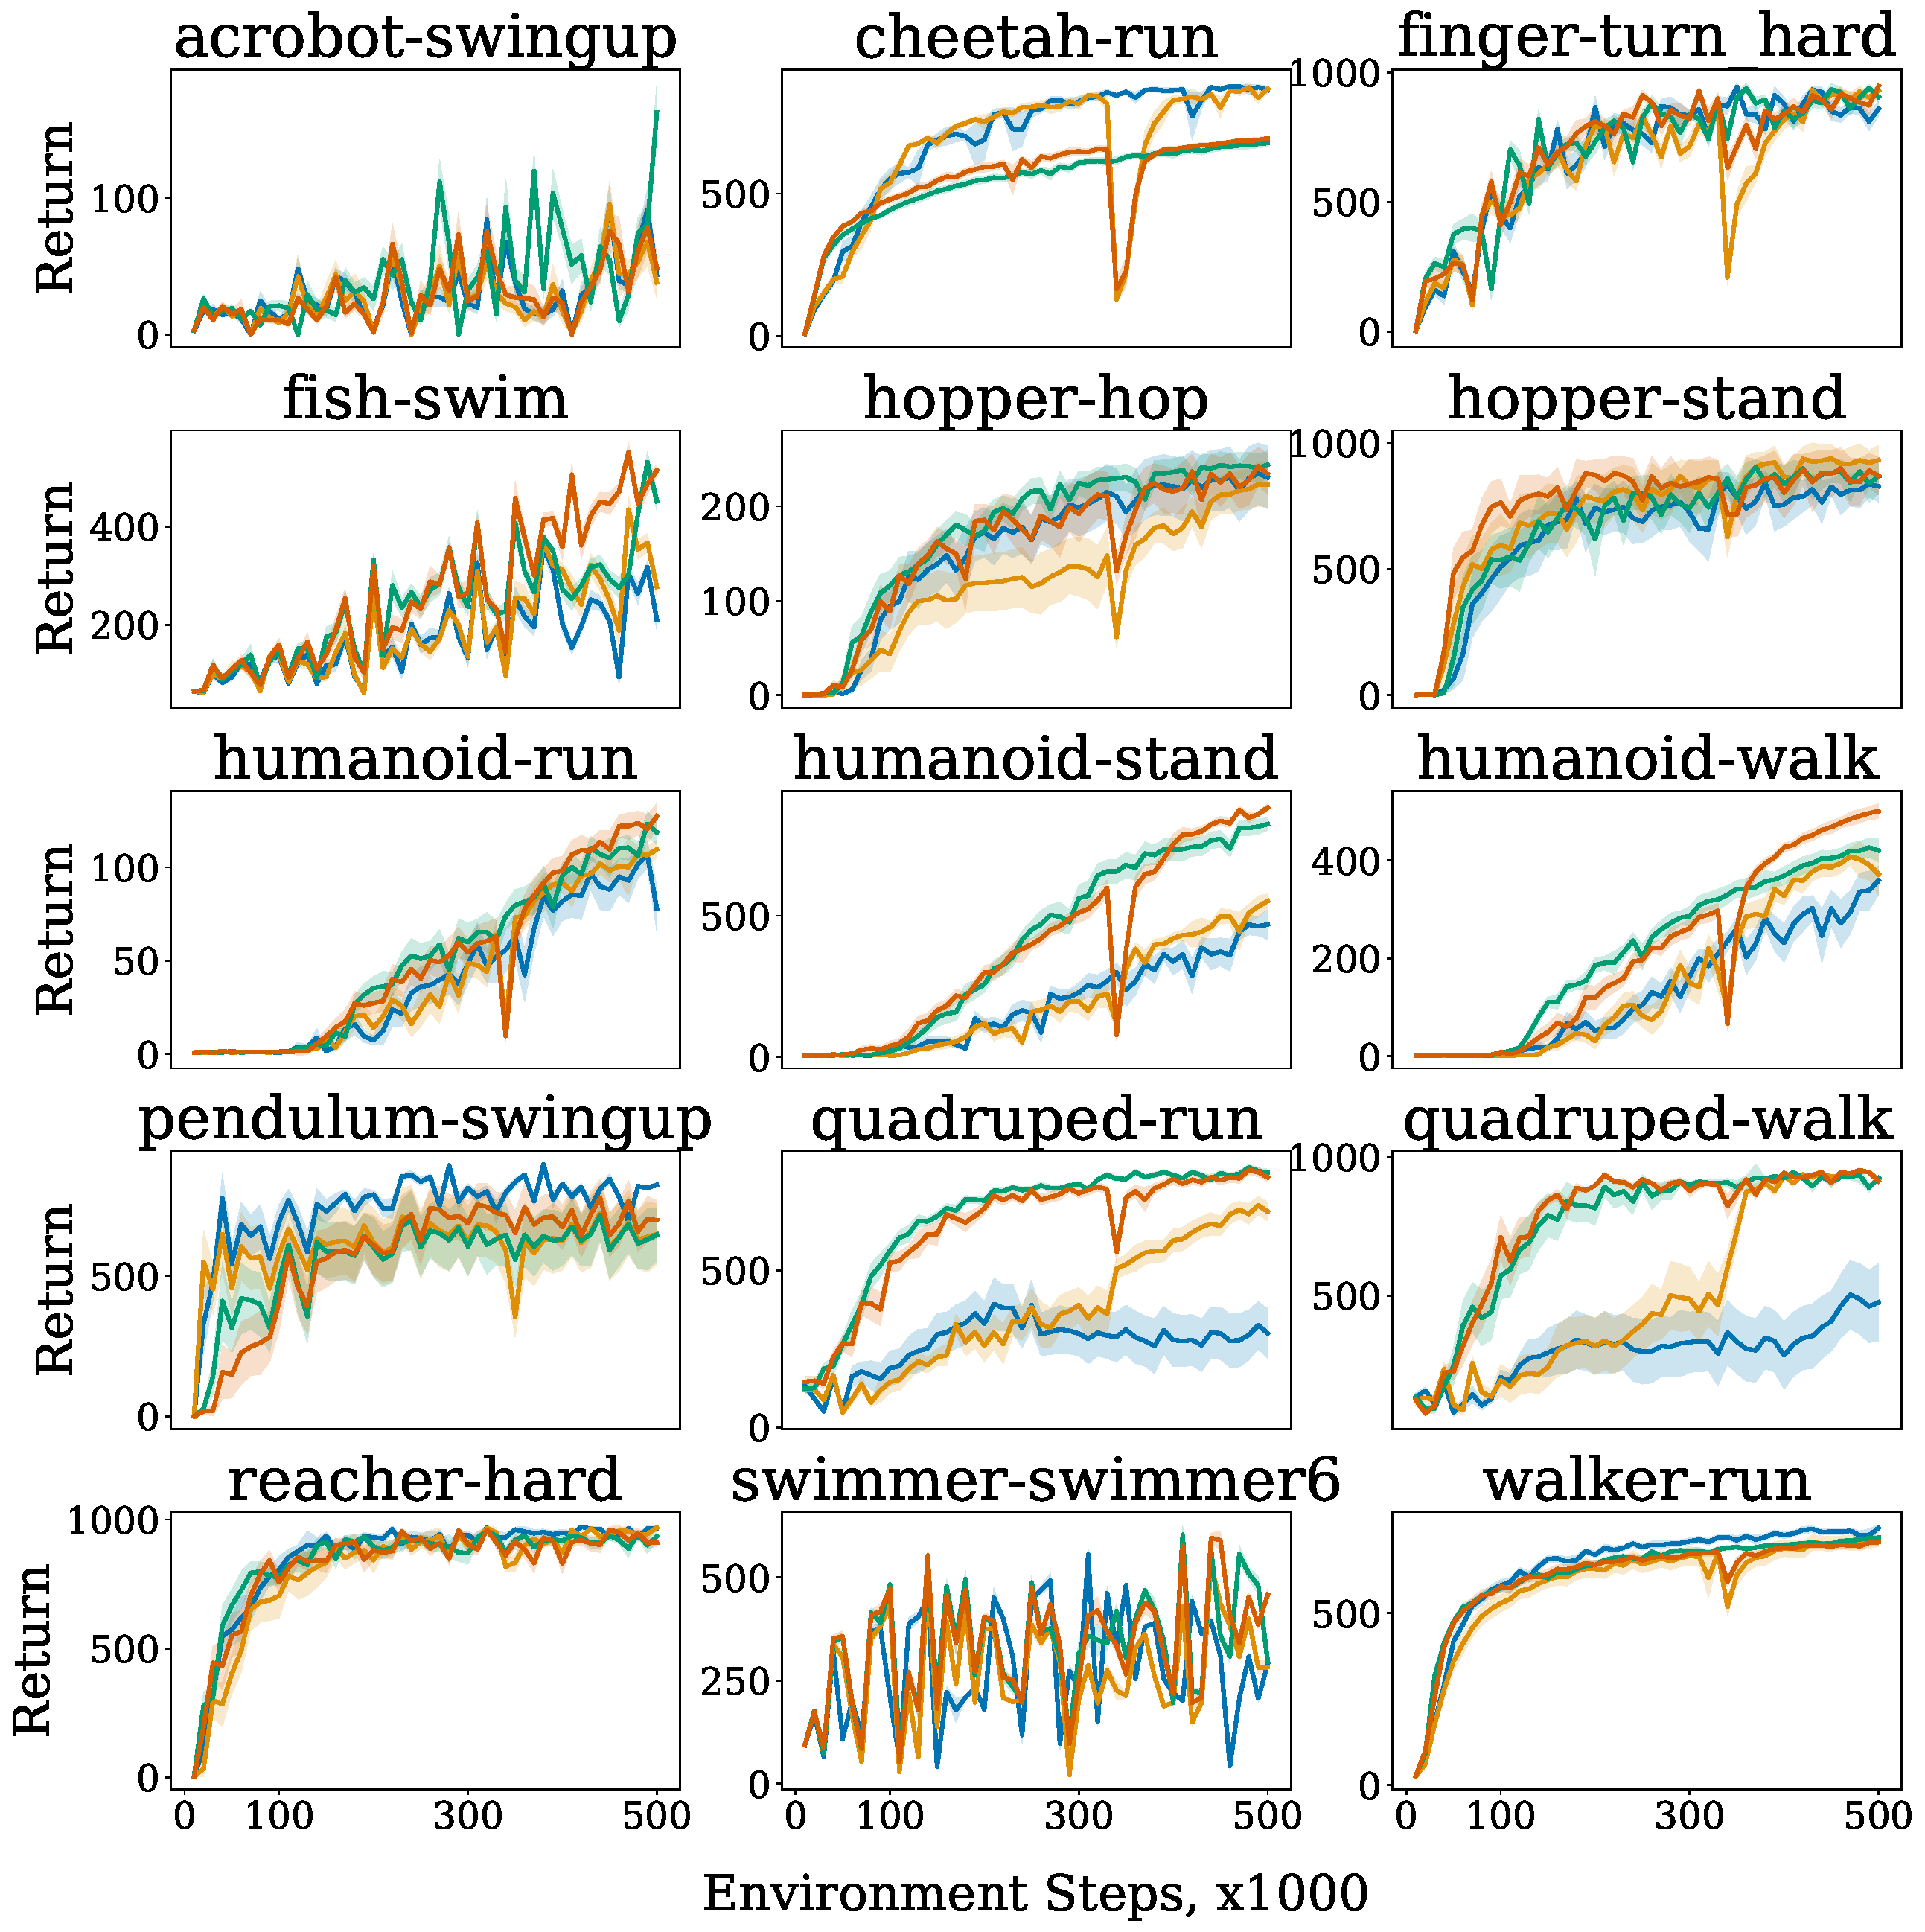
\includegraphics[width=15cm, trim=0cm 0cm 0cm 0cm ,clip]{figures/dissecting/main_exp/utd_8_return.pdf}
    \end{subfigure}%
    \caption{UTD8 Returns on Full DMC15-500K.}
    \label{fig:utd8_ret}
\end{figure}


\begin{figure}[H]
\centering
    \begin{subfigure}[b]{0.8\textwidth}
        \centering
        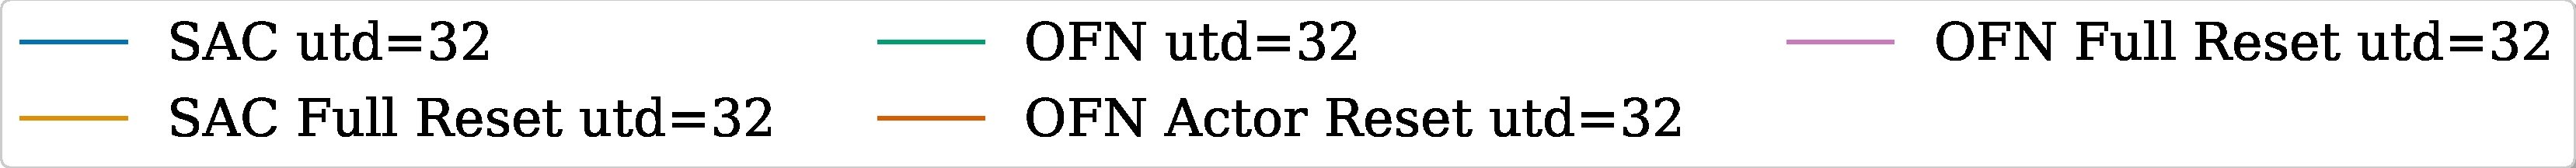
\includegraphics[height=0.8cm]{figures/dissecting/main_exp/utd_32_return_legend.pdf}
    \end{subfigure}\\%
    \begin{subfigure}[b]{1\textwidth}
        \centering
        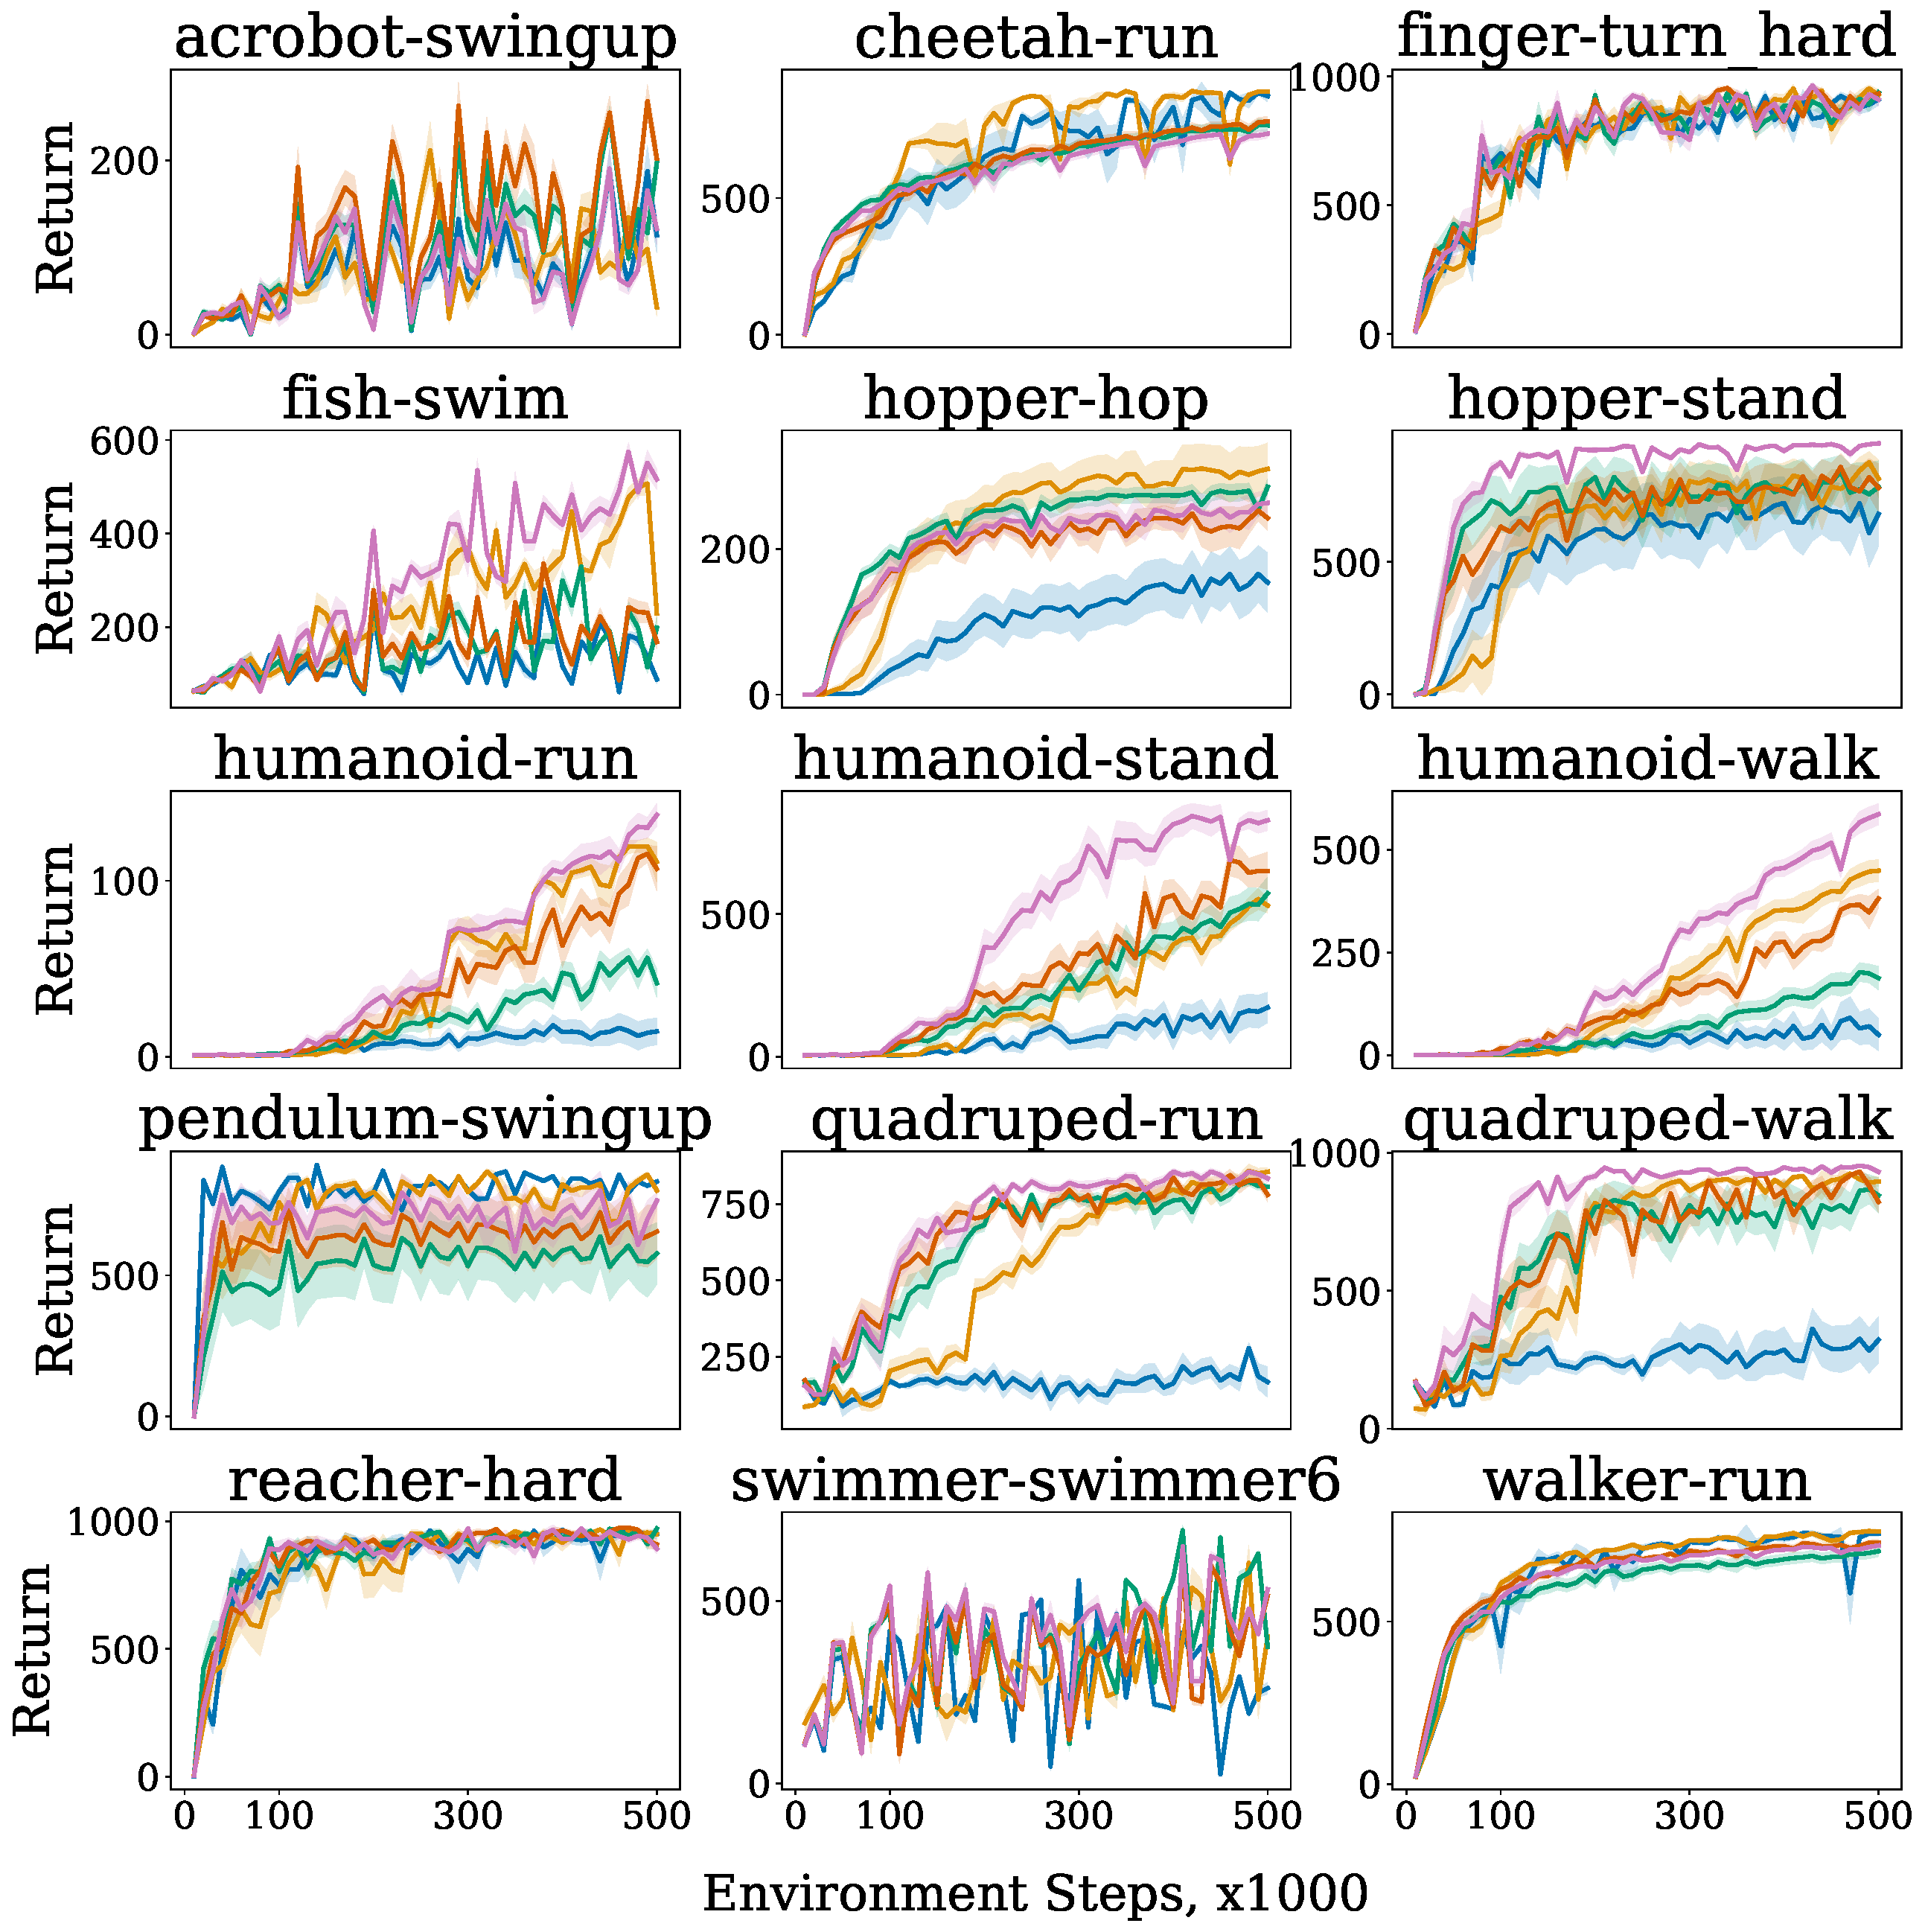
\includegraphics[width=15cm, trim=0cm 0cm 0cm 0cm ,clip]{figures/dissecting/main_exp/utd_32_return.pdf}
    \end{subfigure}%
    \caption{UTD32 Returns on Full DMC15-500K.}
    \label{fig:utd32_ret}
\end{figure}


\subsection{Q-values on all environments} \label{app:exp_q}

\begin{figure}[H]
\centering
    \begin{subfigure}[b]{0.8\textwidth}
        \centering
        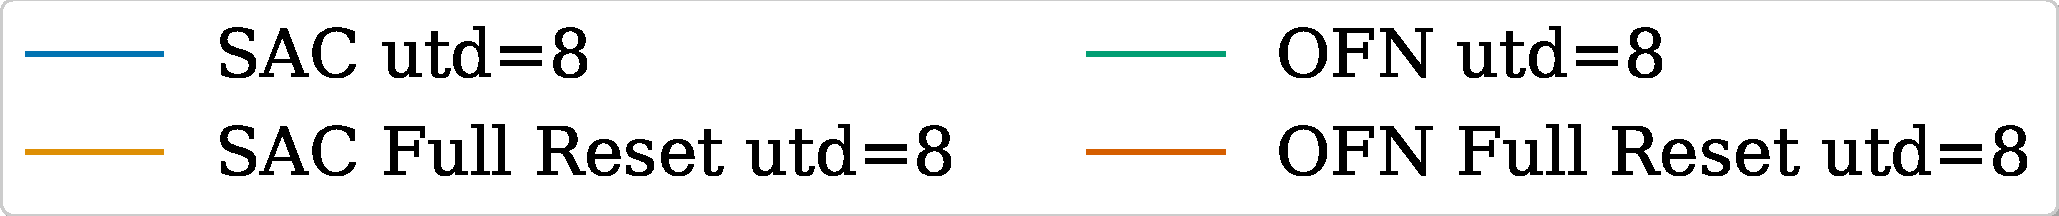
\includegraphics[height=0.8cm]{figures/dissecting/main_exp/utd_8_Q_legend.pdf}
    \end{subfigure}\\%
    \begin{subfigure}[b]{1\textwidth}
        \centering
        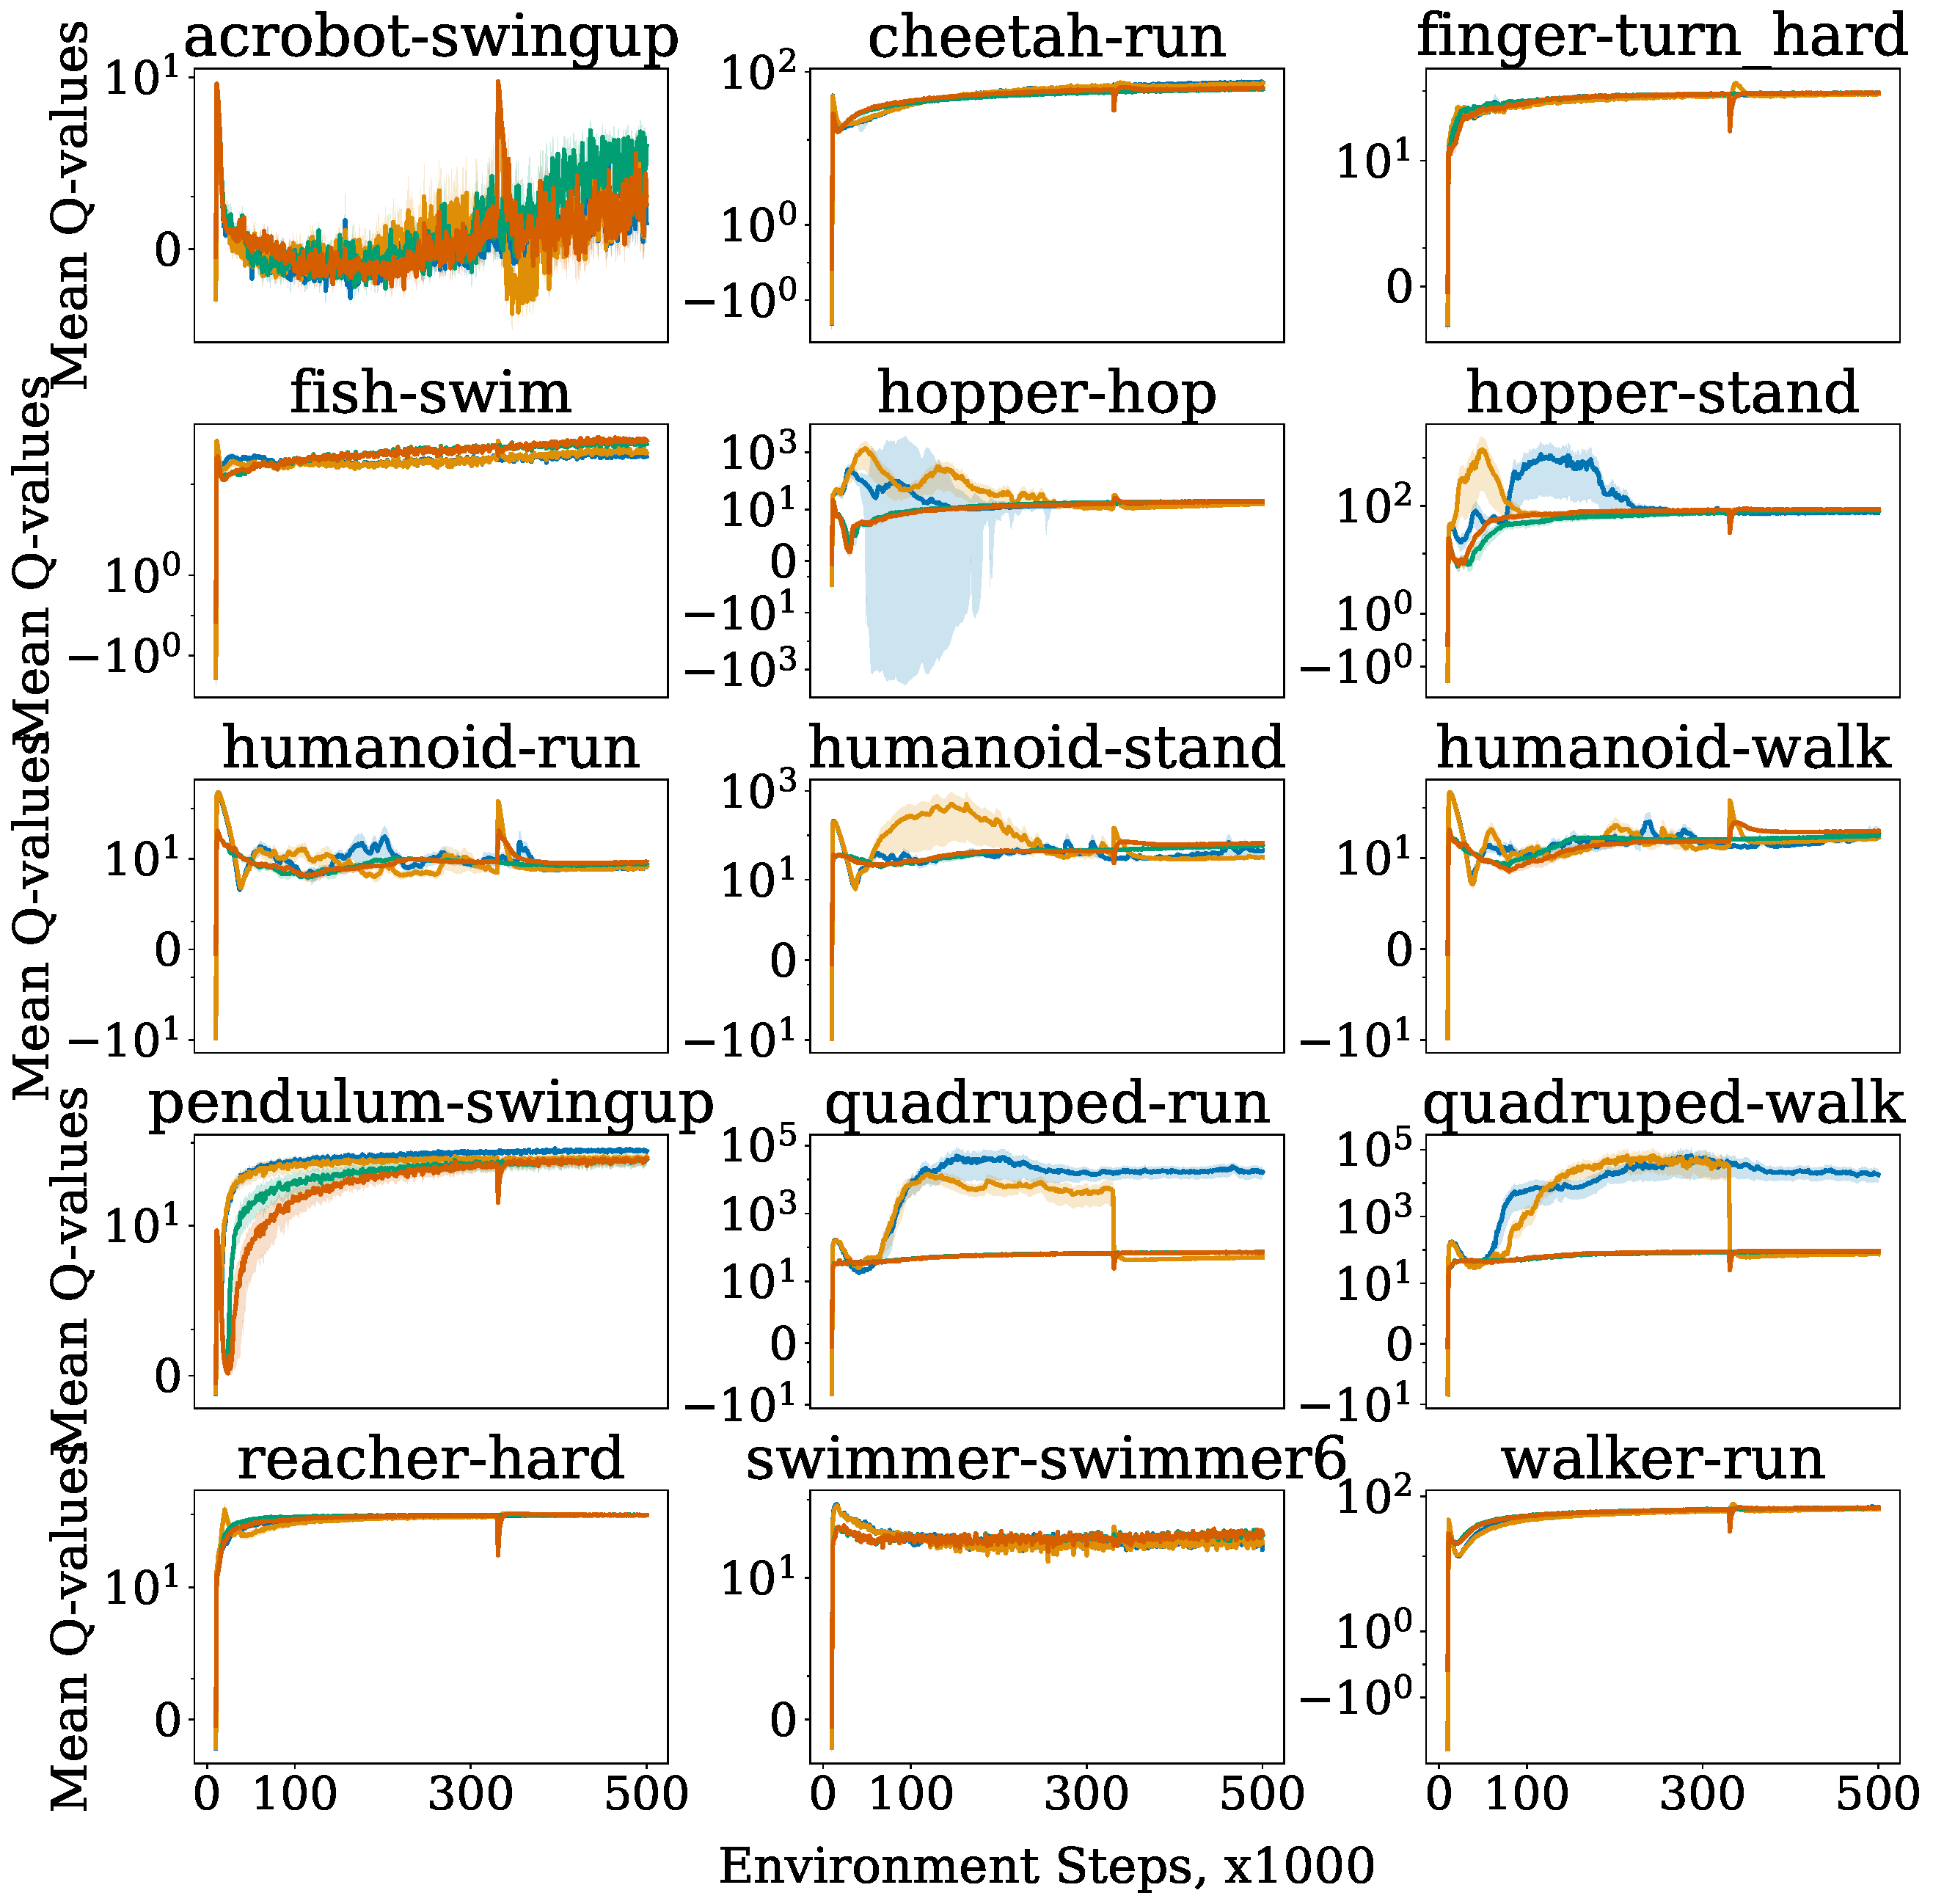
\includegraphics[width=15cm, trim=0cm 0cm 0cm 0cm ,clip]{figures/dissecting/main_exp/utd_8_Q.pdf}
    \end{subfigure}%
    \caption{UTD8 Q-values on Full DMC15-500K. Resetting often works when Q-values diverge. ONF mitigates divergence.}
    \label{fig:utd8_Q}
\end{figure}


\begin{figure}[H]
\centering
    \begin{subfigure}[b]{0.8\textwidth}
        \centering
        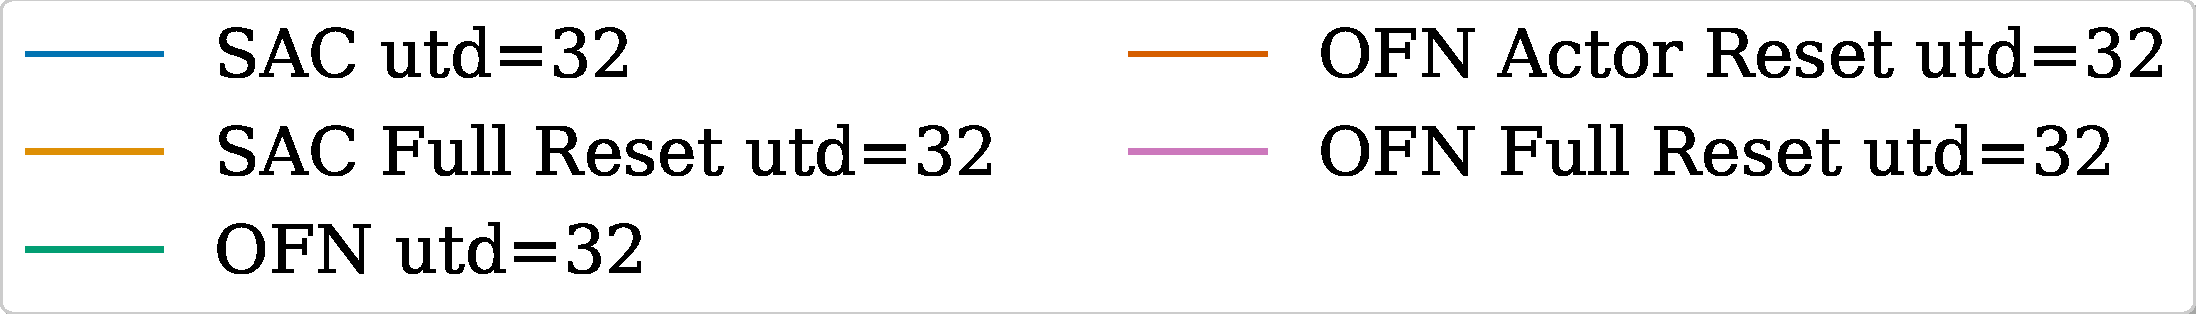
\includegraphics[height=1.1cm]{figures/dissecting/main_exp/utd_32_Q_legend.pdf}
    \end{subfigure}\\%
    \begin{subfigure}[b]{1\textwidth}
        \centering
        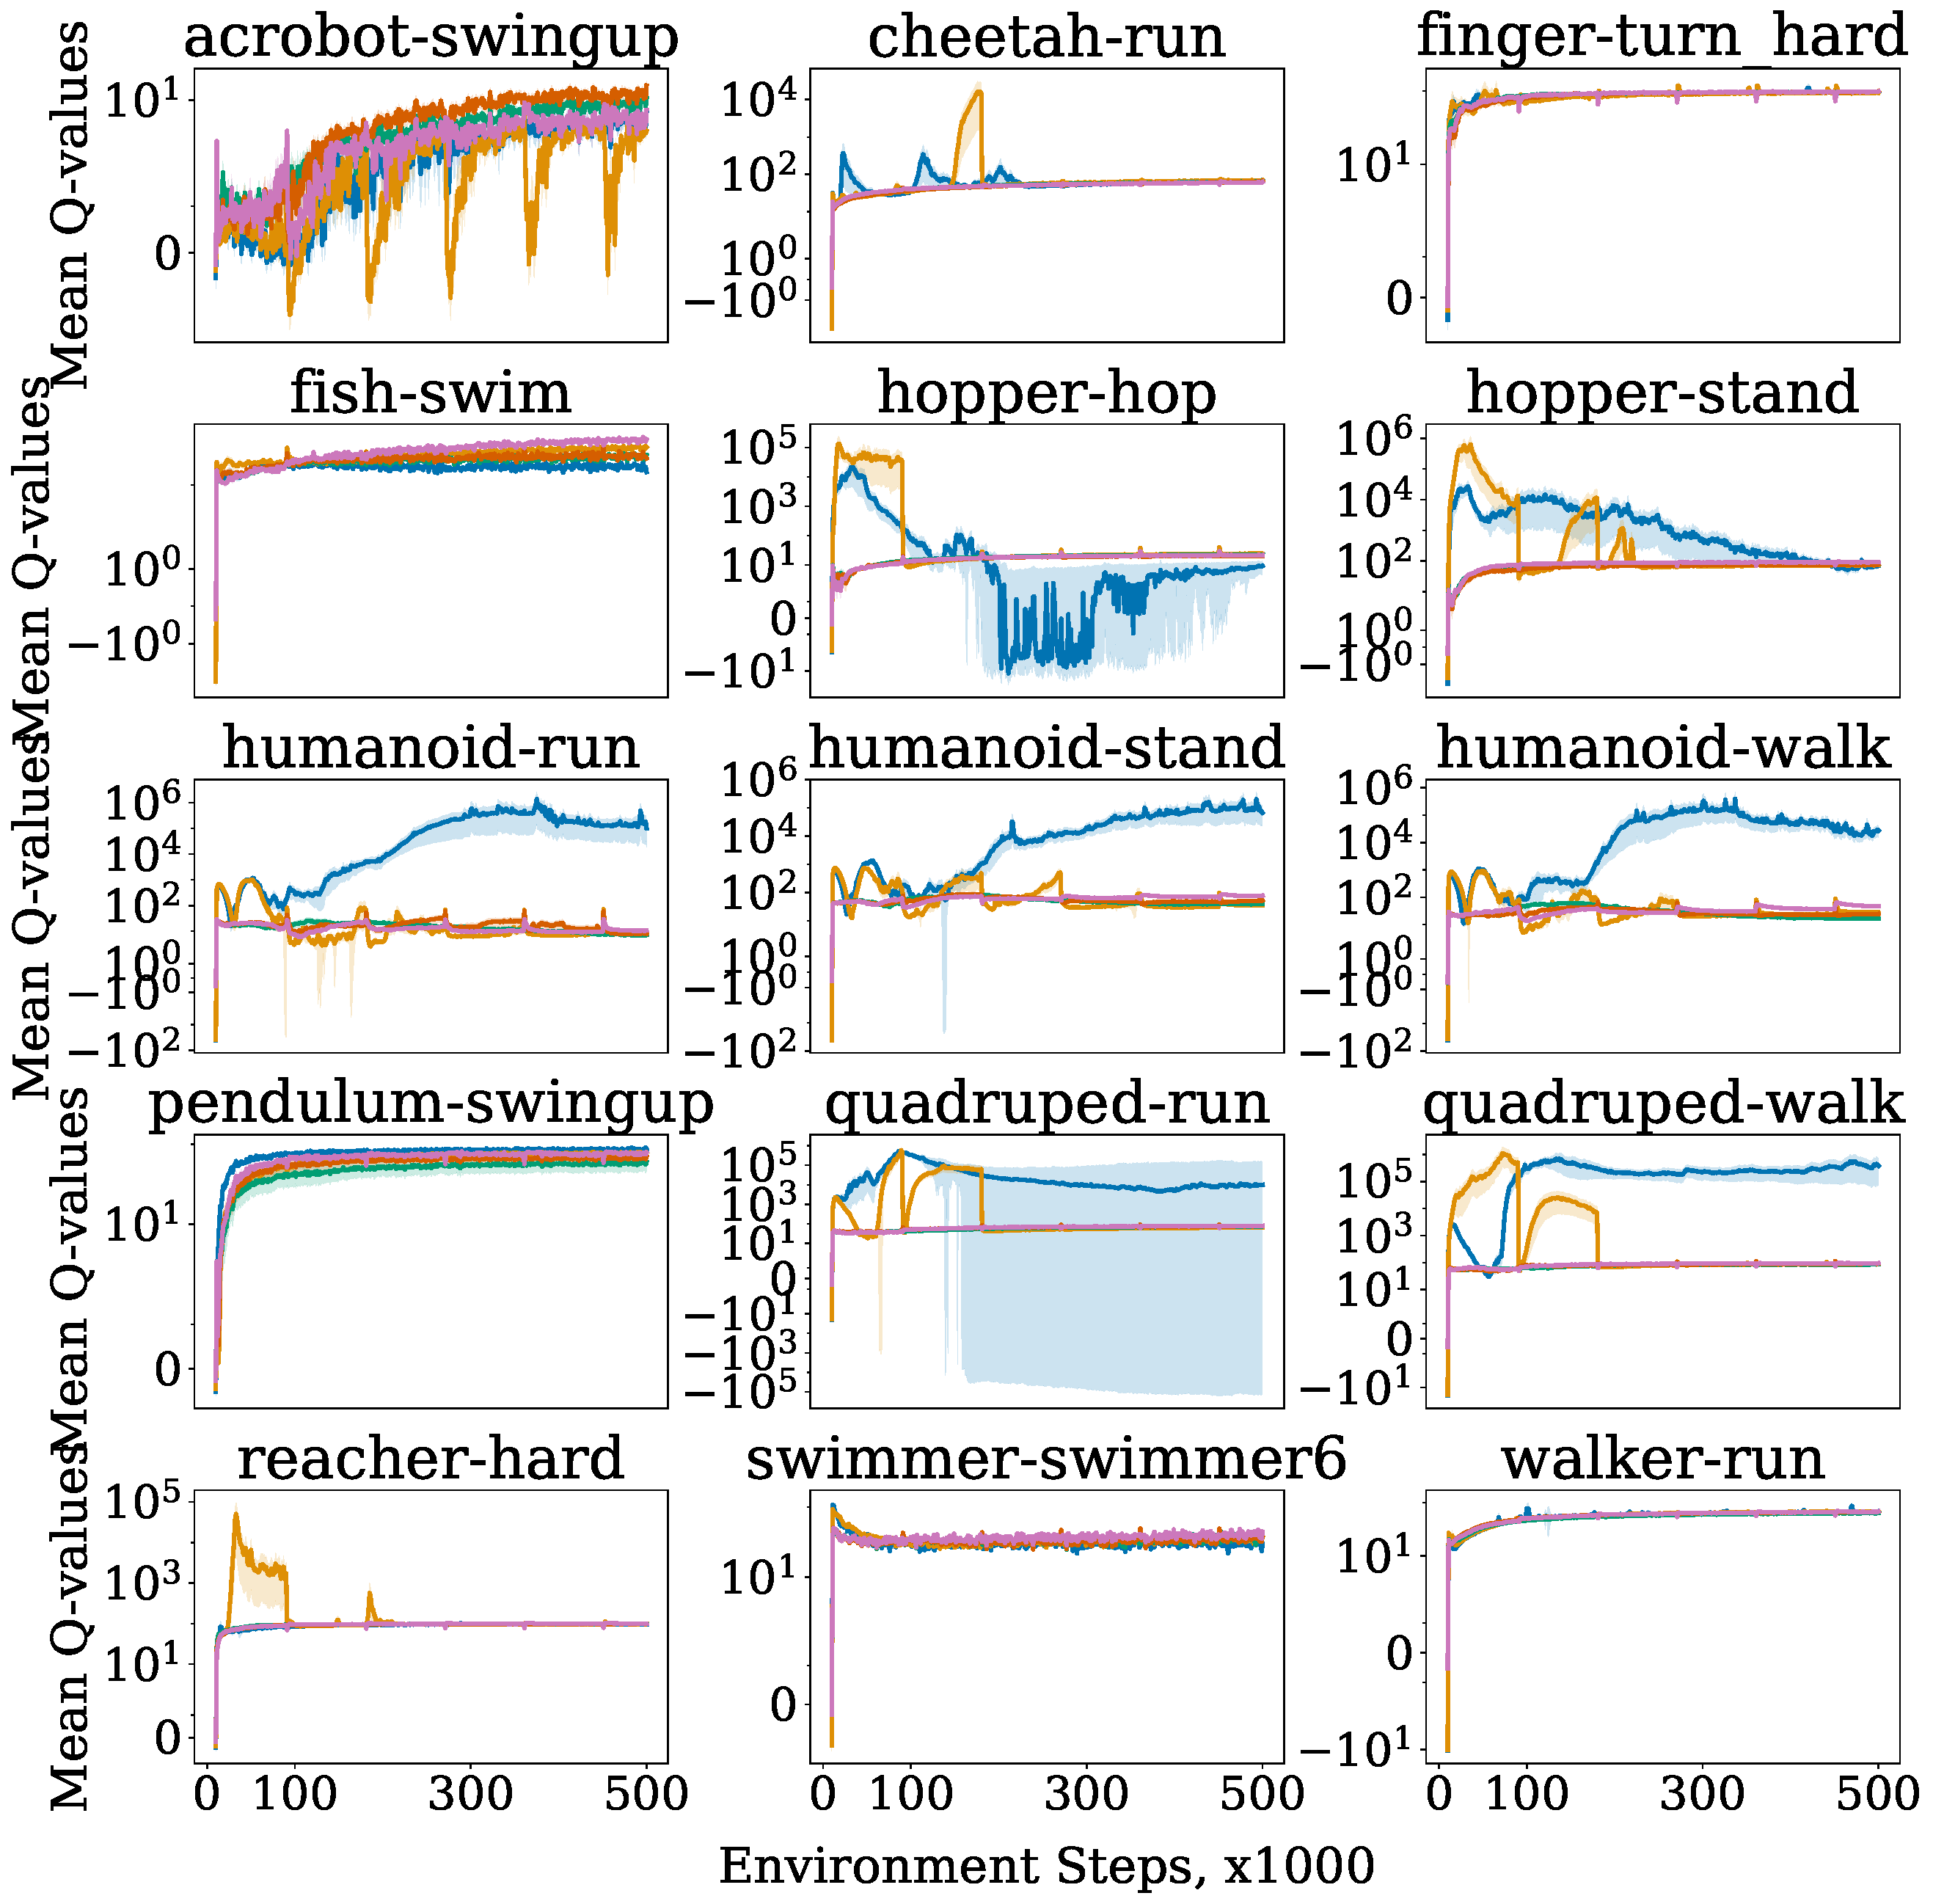
\includegraphics[width=15cm, trim=0cm 0cm 0cm 0cm ,clip]{figures/dissecting/main_exp/utd_32_Q.pdf}
    \end{subfigure}%
    \caption{UTD32 Q-values on Full DMC15-500K. Resetting often works when Q-values diverge. ONF mitigates divergence.}
    \label{fig:utd32_Q}
\end{figure}


\section{Unit norm gradient derivation} \label{app:unitnorm}

Here, we take a look at the gradient of the unit norm projection.

Let $i \in {1, ..., N}$, for all $\mathbf{x} = (x_1, ..., x_n) \in \mathbb{R}^n \setminus \{0\}$. Suppose $f(\mathbf{x}) = \cfrac{\mathbf{x}}{\| \mathbf{x} \|}$. 

Then, 
\begin{align}
    \partial_i f(\mathbf{x}) 
    &= \cfrac{\| \mathbf{x} \| e_i - \mathbf{x} \partial_i \| \cdot \| (\mathbf{x}) }{\|\mathbf{x} \|^2} \\
    &= \cfrac{\| \mathbf{x} \| e_i - \cfrac{x_i}{\|\mathbf{x} \|} \mathbf{x}}{\|\mathbf{x} \|^2} \\
    &= \cfrac{1}{\|\mathbf{x} \|} e_i - \cfrac{x_i}{\|\mathbf{x} \|^3} \mathbf{x}
\end{align}

Note that the second term can grow quite large if the norm of $\mathbf{x}$ is relatively small. Despite this, we are able to remedy the exploding gradients using unit norm projection, likely because gradients are small when the norm is small.

\section{Open Problems and Limitations} \label{app:open}

Feature divergence without regularization is an important problem that contributes substantially to the issues facing high-UTD learning
However, as our experiments show, there are many additional open problems that introducing normalization does not address.

\textbf{Understanding actor issues}~~The resetting experiments in \autoref{fig:overestimation:aggregate} highlight that a part of the performance impact of high UTD comes from the actor optimization, not the critic optimization, as resetting the actor can boost performance without changing the critic.
Our work does not address this issue, and to the best of our knowledge there are no specific attempts to investigate the actor optimization process in deep actor-critic reinforcement learning.

{\bf RL Optimizer}~~ The update dynamics introduced by modern optimizers can exacerbate existing overestimation problems. 
\textcite{dabney2014adaptive} derives adaptive step-sizes for reinforcement learning from a theoretical perspective, but the resulting optimization rules have not been adapted to Deep Reinforcement Learning to the best of our knowledge.
A recent study by \textcite{asadi2023resetting} shows that resetting the optimizer can have some benefit in the DQN setting, where it can be tied to the hard updates of the target Q network.
In addition, \textcite{lyle2023understanding} show that optimizers like Adam can lead to reduced plasticity of neural networks.
However, our experiments also highlight that without the accelerated optimization of modern optimizers, convergence of the Q value can be prohibitively slow, highlighting the urgent need for stable and fast optimization in RL.

{\bf Conservative Learning for Online RL}~~ Most current actor-critic methods use some form of pessimistic value estimate to combat the overestimation bias inherent in off-policy Q learning. i.e. via the use of a twinned Q network \parencite{fujimoto2018addressing}.
However, this can lead to pessimistic under-exploration \parencite{lan2020maxmin}.
To address this, \textcite{moskovitz2021tactical} propose to tune the relative impact of pessimistic and optimistic exploration for the environments, while \textcite{lee2021sunrise} show that by combining independent critic estimates from ensembles, a UBC like exploration bound can be computed.
These changes could be combined with the mitigation strategies for the feature layer divergence in future work to mitigate the harmful effects of under-exploration further.

As our work shows, some of the previous problems with overestimation might not emerge from the bias introduced by off-policy actions, but from the learning dynamics of neural network updates.
This suggests that more work on the exact causes of overestimation might allow us to move beyond the overly pessimistic twinned network minimization trick without needing costly solutions like ensemble methods.

{\bf Tau}~~ The rate of the target network updates is an important hyperparameter in online RL, either through periodic hard copies \parencite{dqn} or the use of a Polyak averaging scheme \parencite{ddpg}.
Updating the network too fast can exacerbate the impact of value divergence, while updating too slowly can delay learning. Preliminary experiments show a relationship between value divergence and target update speed that requires further investigation.

There have also been attempts to accelerate optimization not via the neural network optimization, but through adapting the updates of the target networks \parencite{vieillard2020momentum,farahmand2021pid}.
This is an orthogonal direction to the one presented here, and the interplay between target network updates and neural network optimization steps are an important topic for future work.


{\bf Reward Shaping Impact}~~ In several environments, we observe almost no detrimental effects due to high update ratios, while in others the Q-values diverge even without moving beyond one update per sample collected.
A closer inspection suggests that environments in which the initial reward is small and uninformative are much more prone to lead to catastrophic divergence, suggesting a close connection between reward shaping and divergence.
While sparse reward problems have received much attention in the context of exploration, our findings suggests that they also present a challenge for efficient optimization.
Beyond this phenomenon, the interactions between optimization and explorations have been hypothesized to be a strong contributing factor to the good performance of some algorithms \parencite{schaul2022phenomenon}, but the role diverging Q-values play in this phenomenon is to the best of our knowledge mostly unexplored.



